\section{Auswertung und Diskussion}
\label{sec:AuswertungDiskussion}

\subsection*{Bestrahlungsplan für das PTV1}
Bei der ersten Bestrahlungsserie wird das PTV1 bestrahlt. In den Abbildungen \ref{fig:lunge1x}, \ref{fig:lunge1y} und \ref{fig:lunge1z}
ist die Dosisverteilung in der Lunge in der
Transversal-, Sagittal- und Frontalansicht zu sehen. In den Abbildungen ist zu erkennen, dass die $\SI{95}{\percent}$ Isodosenlinie das
rot eingezeichnete PTV in dem meisten Bereichen gut umschließt.
Für eine bessere Beurteilung ist das Dosis-Volumen-Histogramm in der Abbildung \ref{fig:lunge1dvh} gezeigt.
Anhand der DVH Kurve für das PTV1 (rot) ist zu erkennen, dass lediglich in einem kleinen Teil des PTVs es
nicht gelungen ist eine Dosis von $\SI{95}{\percent}$ zu erreichen.
Das liegt daran, dass das PTV1 bis in die Lunge hineinreicht, die hauptsächlich aus Luft besteht.
Da Luft eine geringere Dichte als das Tumorgewebe hat, wird dort weniger Dosis absorbiert und somit konnte in diesen Bereichen des PTVs nicht
die gewünschte Dosis von $95\%$ erreicht werden.
Aus diesem Grund liegt die minimale Dosis, die im PTV1 deponiert wird, bei $\SI{86.2}{\percent}$.
Es werden trotzdem $\SI{95,25}{\percent}$ des Volumens des PTVs von der $\SI{95}{\percent}$ Isodosenlinie umschlossen.
Die maximale relative Dosis $\SI{105.3}{\percent}$ wird im PTV1 deponiert und liegt $\SI{1.7}{\percent}$ unter der
erlaubten maximalen Dosis von $\SI{107}{\percent}$ \cite{ICRU}.


\begin{figure}[H]
	\centering
	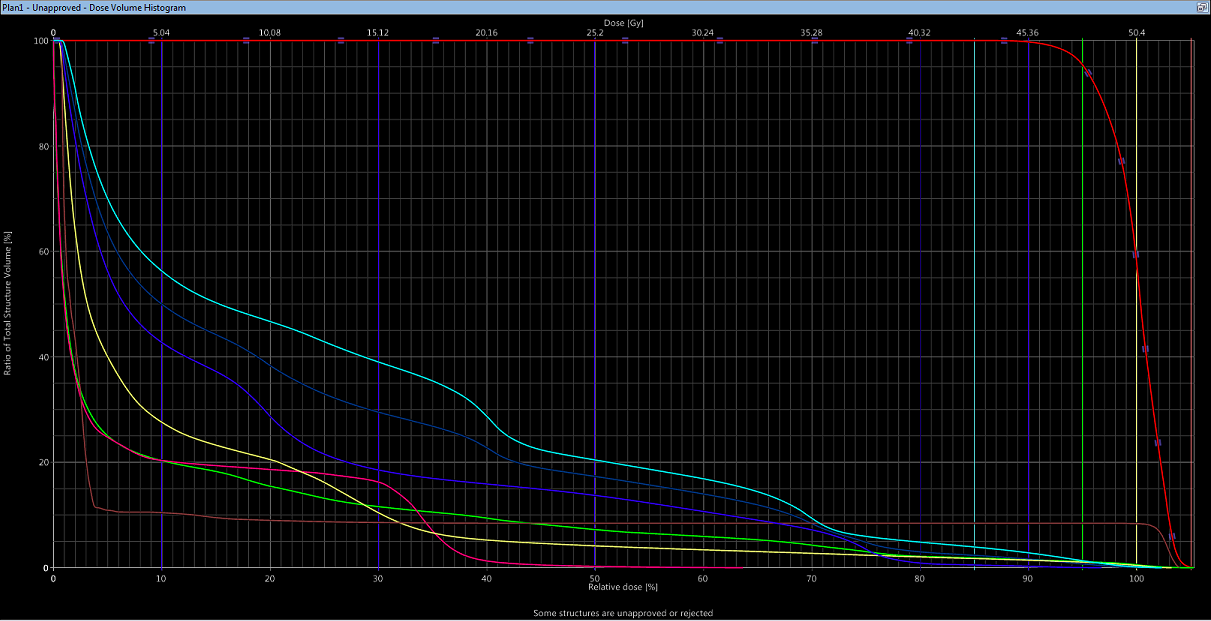
\includegraphics[width=\linewidth]{Bilder/Lunge1_DVH}
	\caption{Zu sehen ist das DVH der Lunge. In roter Farbe dargestellt ist das PTV1 und in grüner Farbe der Thorax. Außerdem sind noch die einzelnen Isodosenlinien eingezeichnet und die einzelnen Kurven zu den Risikoorgane wie Herz (gelb), Lunge rechts (hellblau), Lunge links (blau), Lunge gesamt (dunkelblau), die Speiseröhre (braun) und das Rückenmark (pink).}
	\label{fig:lunge1dvh}
\end{figure}

Anhand des DVHs des gesamten Thorax (grüne Kurve) ist zu erkennen, dass in dem gesamten Thorax nur eine relativ geringe Dosis deponiert wird.
Etwa $\SI{7,22}{\percent}$ des Thoraxvolumens erhält noch eine relative Dosis von $\SI{50}{\percent}$.
Durch die DVH Kurven der Risikoorgane ist zu erkennen, dass diese gut geschont werden konnten.
Von den Risikoorganen erhält die Lunge die meiste Dosis, was bei der Lokalisation des Tumors zu erwarten war.
Um zu überprüfen ob die Organdosisgrenzwerte eingehalten worden sind, müssen beide Bestrahlungspläne betrachtet werden.
Aus diesem Grund wird die Dosisverteilung der Risikoorgane am Ende des Protokolls genauer untersucht.

\begin{figure}[H]
	\centering
	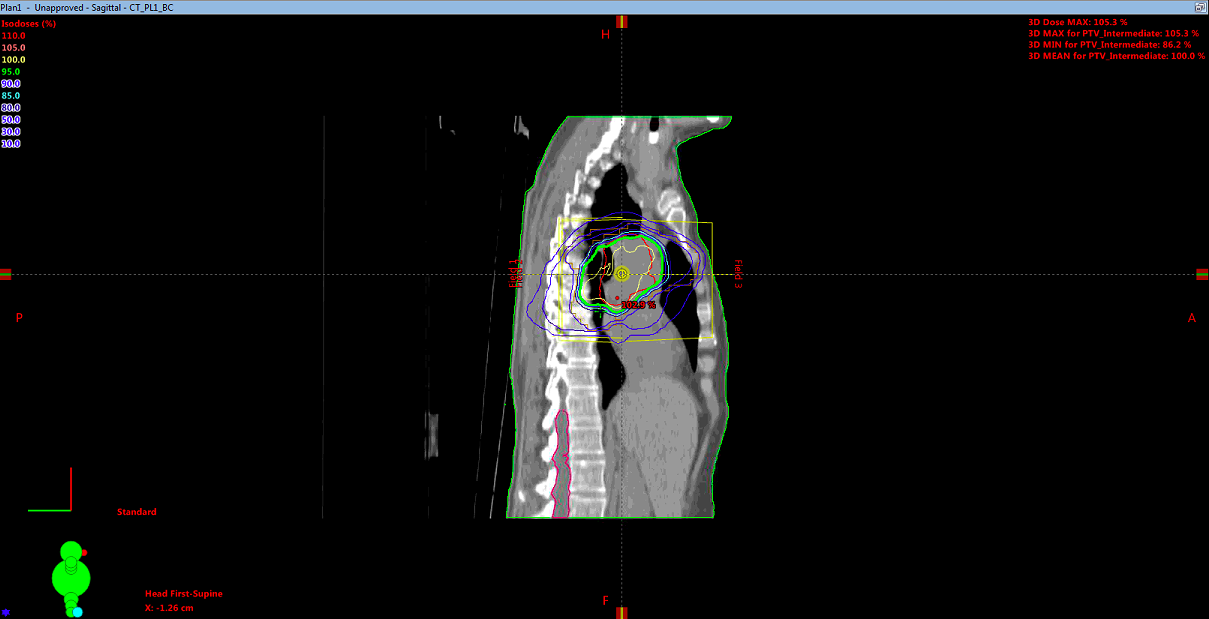
\includegraphics[width=\linewidth]{Bilder/Lunge1_X}
	\caption{Darstellung der Dosisverteilung in der Sagittalansicht der Lunge.}
	\label{fig:lunge1x}
\end{figure}

\begin{figure}[H]
	\centering
	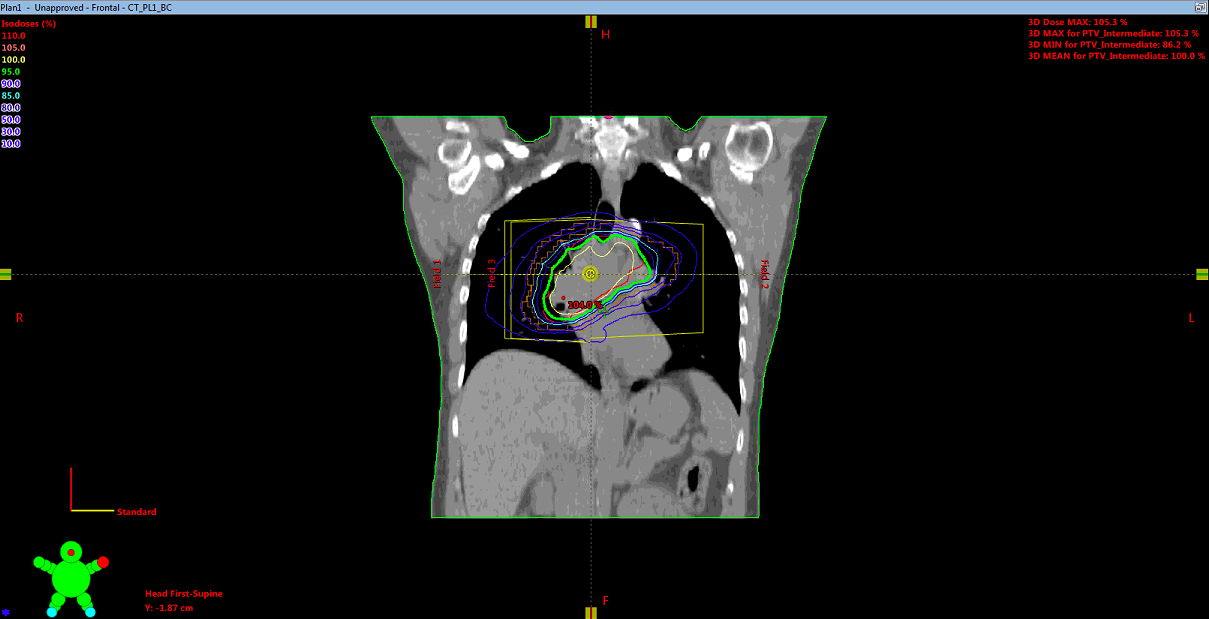
\includegraphics[width=\linewidth]{Bilder/Lunge1_Y}
	\caption{Darstellung der Dosisverteilung in der Frontalansicht  der Lunge.}
	\label{fig:lunge1y}
\end{figure}

\begin{figure}[H]
	\centering
	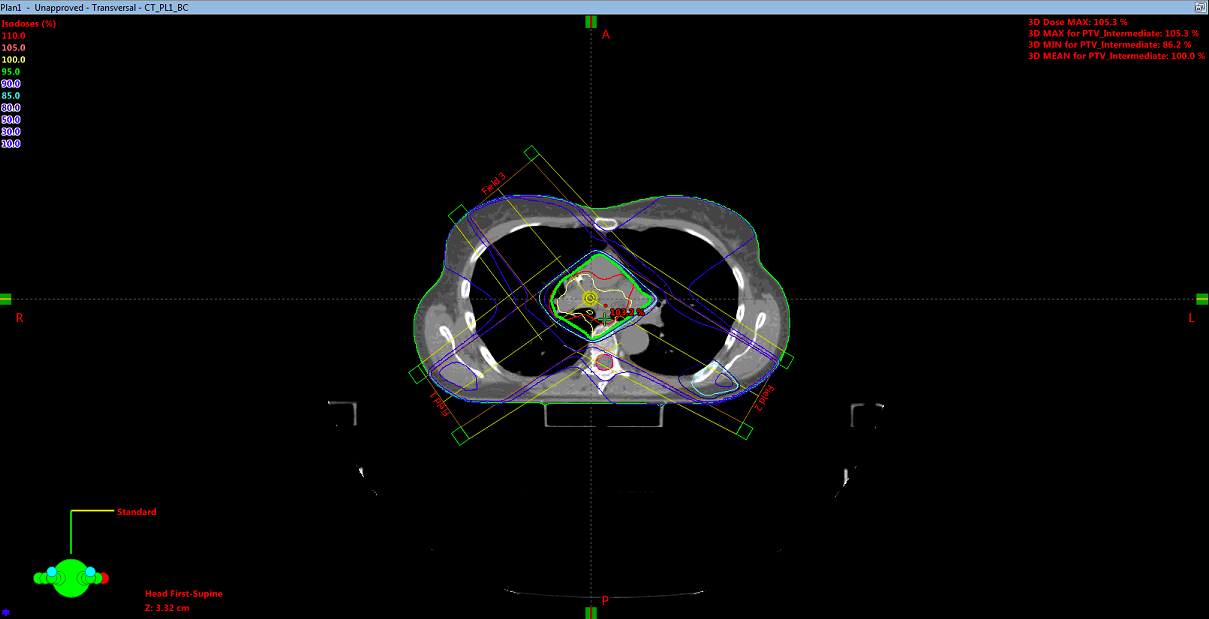
\includegraphics[width=\linewidth]{Bilder/Lunge1_Z}
	\caption{Darstellung der Dosisverteilung in der Transversalansicht  der Lunge.}
	\label{fig:lunge1z}
\end{figure}

\subsection*{Bestrahlungsplan für das PTV2}

Bei dem zweiten Bestrahlungsplan wird das kleinere PTV2 bestrahlt.
Die resultierende Dosisverteilung ist in den Abbildungen \ref{fig:lunge2x}, \ref{fig:lunge2y}
und \ref{fig:lunge2z} gezeigt. Dabei sind die gleichen Ansichten gezeigt, wie bei dem ersten Plan.
Auch hier ist es nicht gelungen, dass die $\SI{95}{\percent}$ Isodosenlinie das PTV2 komplett umschließt.
Es werden $\SI{94,1}{\percent}$ des Volumens von der $\SI{95}{\percent}$ Isodosenlinie umschlossen.
Auch in diesem Fall liegt es an den großen Dichteunterschied zwischen Lungengewebe und Tumorgewebe.
Die maximale relative Dosis wird innerhalb des PTVs appliziert und liegt bei $\SI{106.3}{\percent}$,
was unterhalb der erlaubten maximalen Dosis von $\SI{107}{\percent}$ liegt. Die minimale relative Dosis in dem PTV2 liegt bei $\SI{87.3}{\percent}$.
Diese Dosis liegt minimal unterhalb des gewünschten Dosis von $\SI{95}{\percent}$.
Das zugehörige DVH ist in der Abbildung \ref{fig:lunge2dvh} gezeigt.

\begin{figure}[H]
	\centering
	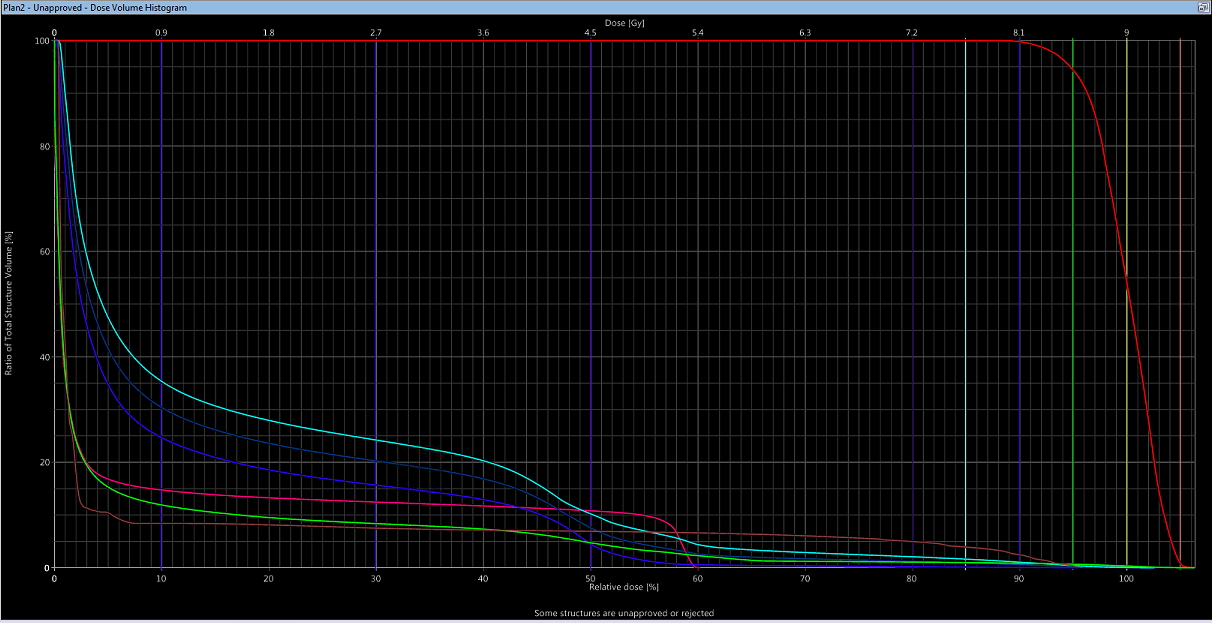
\includegraphics[width=\linewidth]{Bilder/Lunge2_DVH}
	\caption{Zu sehen ist das DVH der Lunge. In roter Farbe dargestellt ist das PTV2 und in grüner Farbe ist der gesamte Thorax. Außerdem sind noch die einzelnen Isodosenlinien eingezeichnet und die einzelnen Kurven zu den Risikoorgane wie z.B. Herz (gelb), Lunge rechts (hellblau), Lunge links (blau), Lunge gesamt (dunkelblau), die Speiseröhre (braun) und das Rückenmark (pink).}
	\label{fig:lunge2dvh}
\end{figure}

Anhand des DVHs des gesamten Thorax (grüne Kurve) ist zu erkennen, dass in dem gesamten Thoraxvolumen nur eine relativ geringe Dosis deponiert wird.
Nur etwa $\SI{4,58}{\percent}$ des Volumens erhält noch eine relative Dosis von $\SI{50}{\percent}$.
Auch bei diesen Plan sind die Risikoorgane gut geschont worden, was anhand ihrer DVH Kurven gesehen werden kann.
Im folgenden wird die Summe der beiden Pläne betrachtet um beurteilen zu können ob die Organdosisgrenzwerte eingehalten worden sind.

\begin{figure}[H]
	\centering
	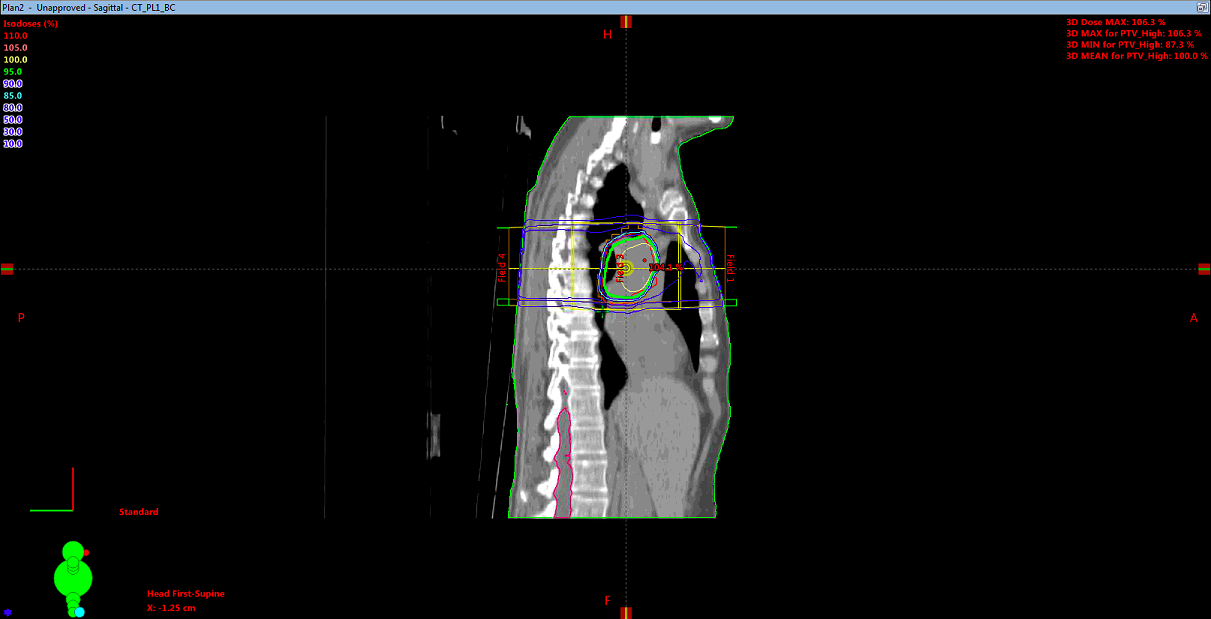
\includegraphics[width=\linewidth]{Bilder/Lunge2_X}
	\caption{Darstellung der Dosisverteilung in der Sagittalansicht der Lunge.}
	\label{fig:lunge2x}
\end{figure}

\begin{figure}[H]
	\centering
	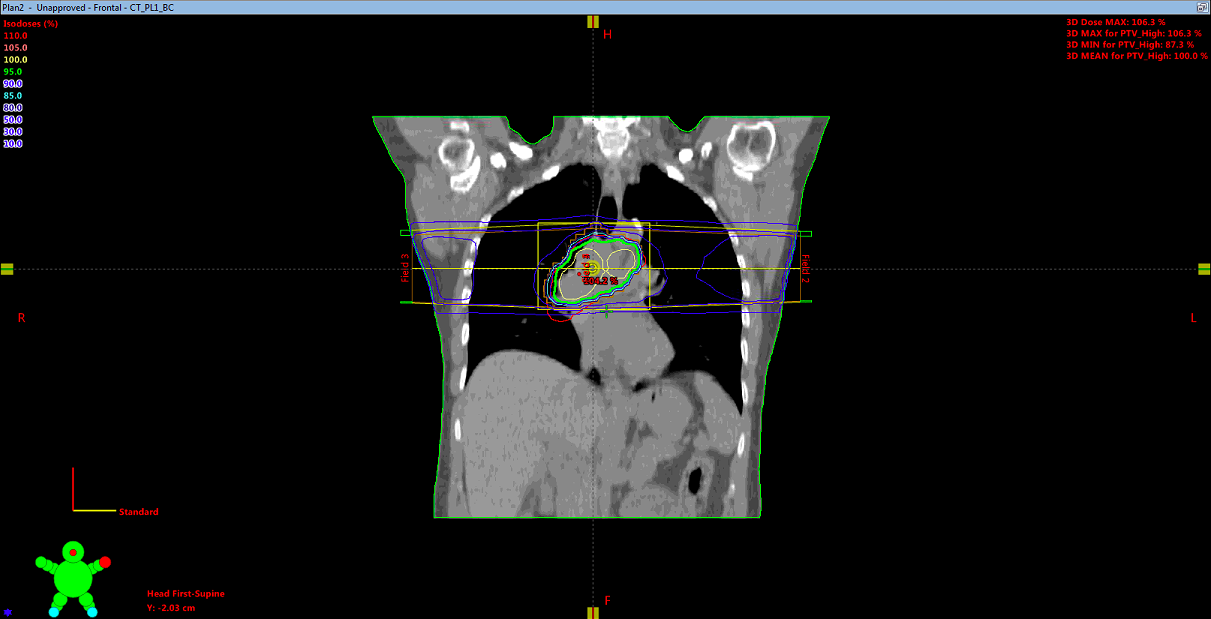
\includegraphics[width=\linewidth]{Bilder/Lunge2_Y}
	\caption{Darstellung der Dosisverteilung in der Frontalansicht der Lunge.}
	\label{fig:lunge2y}
\end{figure}

\begin{figure}[H]
	\centering
	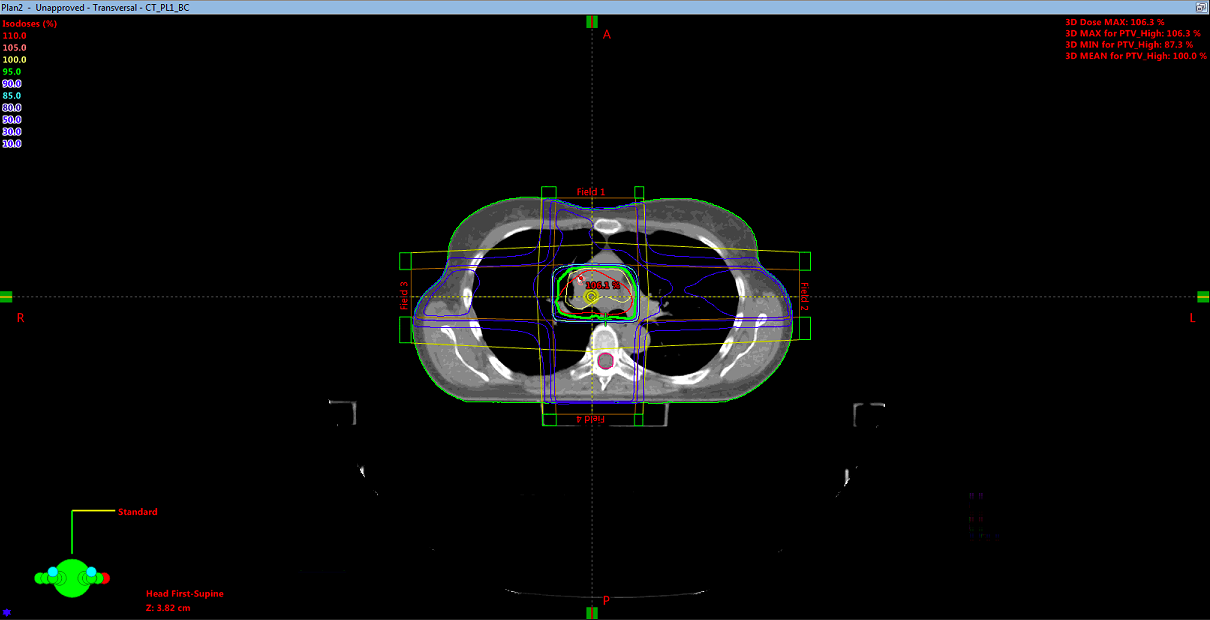
\includegraphics[width=\linewidth]{Bilder/Lunge2_Z}
	\caption{Darstellung der Dosisverteilung in der Transversalansicht der Lunge.}
	\label{fig:lunge2z}
\end{figure}


\subsection*{Summe der Bestrahlungspläne}

In der Abbildung \ref{fig:lunge2dvh} ist das DVH der Summe der beiden Bestrahlungspläne dargestellt.
Die Organdosisgrenzwerte werden aus der QUANTEC Tabelle entnommen. Die mittlere Dosis der Lunge darf $\SI{20}{\gray}$ nicht überschreiten
und es darf nicht mehr als $\SI{30}{\percent}$ des Lungenvolumens eine Dosis von $\SI{20}{\gray}$ erhalten \cite{grenz}.
Diese Grenzwerte wurden erfolgreich eingehalten, weil nur $\SI{25.76}{\percent}$ des Volumens eine Dosis von $\SI{20}{\gray}$ erhält und die mittlere Dosis
liegt bei $\SI{12.717}{\gray}$.
Der Grenzwert für die mittlere Dosis bei dem Herz beträgt $\SI{26}{\gray}$ und weniger als $\SI{46}{\percent}$ des Herzvolumens darf
eine Dosis von $\SI{30}{\gray}$ erhalten \cite{grenz}. Dies wurde auch erfolgreich eingehalten, weil nur $\SI{3.7}{\percent}$ mit einer Dosis von
$\SI{30}{\gray}$ bestrahlt wird und die mittlere Dosis liegt bei $\SI{5.894}{\gray}$.
Bei dem Rückenmark darf die maximale Dosis $\SI{45}{\gray}$ nicht überschreiten \cite{grenz}.
Bei diesen Plänen liegt die maximale Dosis des Rückenmarks bei $\SI{31.92}{\gray}$ und liegt somit unterhalb des Grenzwertes.
Bei dem Oesophagus darf die mittlere Dosis $\SI{34}{\gray}$ nicht überschreiten und weniger als $50\%$ des Volumens darf eine Dosis von $\SI{35}{\gray}$
erhalten \cite{QUANTEC}. Auch diese Grenzwerte wurden eingehalten, da die mittlere Dosis bei $\SI{5.940}{\gray}$ liegt und nur etwa $9\%$ des Volumens eine
Dosis von $\SI{35}{\gray}$ erhält. \\

Bei den erstellten Plänen konnte zwar nicht erreicht werden, dass die PTVs komplett von der $95\%$ Isodosenlinie
umschlossen werden, allerdings ist der Anteil der PTVs der nicht umschlossen werden konnte sehr gering.
Durch die verwendeten Felder mit individuell angepassten MLCs konnten die Organdosisgrenzwerte aller Risikoorgane eingehalten werden.

\begin{figure}[H]
	\centering
	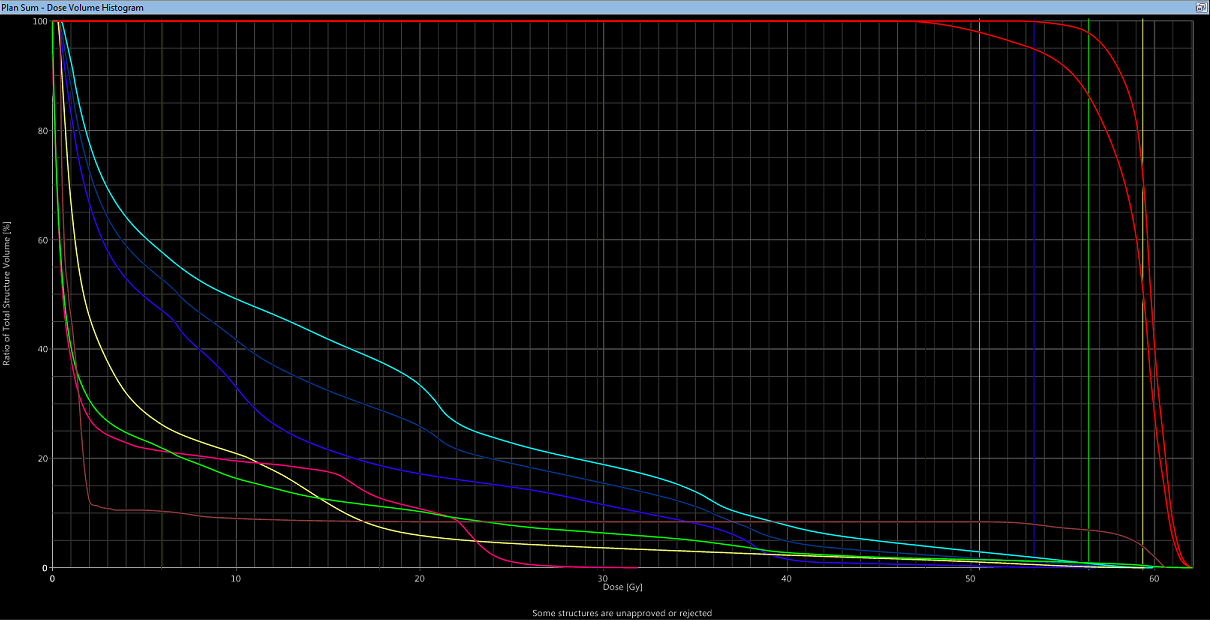
\includegraphics[width=\linewidth]{Bilder/Lunge_DVHsum}
	\caption{DVH für die Summe der beiden Bestrahlungspläne. Für das PTV1 und PTV2 in rot und den gesamten Körper in grün. Außerdem ist das DVH für das Herz in gelb, für die Lunge in dunkelblau, für die Speiseröhre in braun und für das Rückenmark in pink.}
	\label{fig:lungedvhsum}
\end{figure}
